\documentclass[seminarski, times, utf8]{fer}


\usepackage{blindtext}
\usepackage{indentfirst}
\usepackage{graphicx}
\usepackage{float}
\usepackage{subfigure}

%--- PODACI O RADU / THESIS INFORMATION ----------------------------------------

% Naslov na engleskom jeziku / Title in English
\title{Deepfake detection using GAN}

% Naslov na hrvatskom jeziku / Title in Croatian
\title{Detekcija uvjerljivog krivotvorenog sadržaja na društvenim mrežama uporabom GAN-ova}

% Autor / Author
\author{Barbara Kos, Matija Pavlović}

\voditelj{prof. dr. sc. Tomislav Hrkać}

% Datum rada na engleskom jeziku / Date in English
\date{}

% Datum rada na hrvatskom jeziku / Date in Croatian
\date{}

%-------------------------------------------------------------------------------


\begin{document}


% Naslovnica se automatski generira / Titlepage is automatically generated
\maketitle


%--- SAŽETAK / ABSTRACT --------------------------------------------------------

% Sažetak na hrvatskom
\begin{sazetak}
Ovaj seminarski rad predstavlja metodu detekcije uvjerljivog krivotvorenog sadržaja na društvenim mrežama uporabom GAN-ova. Prvo se detaljno razrađuje sam pojam uvjerljivog krivotvorenog sadržaja, njegova pojava i opasnosti koje proizlaze iz te pojave.
Nadalje se definiraju osnovni pojmovi i koncepti GAN-ova, predlaže se implementacija sustava koji obavlja detekciju, razmatraju se prednosti i nedostatci implementiranog sustava u odnosu na druge načine detekcije. 
Naposljetku, iznose se i prijedlozi budućeg rada na projektu, moguća unaprjeđenja i iznose se zaključci o izvedivosti implementacije predloženog sustava u stvarnosti.
\end{sazetak}

\begin{kljucnerijeci}
deepfake, detekcija, GAN, strojno učenje, duboko učenje
\end{kljucnerijeci}

% Sažetak na engleskom
\begin{abstract}
This seminar paper presents a method of detecting persuasive fake content on social networks using GANs. First, the notion of persuasive fake content itself, its phenomenon and the dangers arising from it are discussed in detail. 
Furthermore, the basic concepts and concepts of GANs are defined, the implementation of a detection system is proposed, the advantages and disadvantages of the implemented system compared to other detection methods are discussed. 
In conclusion, we discuss future work, improvements and feasability of a real world implementation.
\end{abstract}

\begin{keywords}
 deepfakes, detection, GAN, ML, deep learning
\end{keywords}


% Sadržaj se automatski generira / Table of contents is automatically generated
\tableofcontents


%--- UVOD / INTRODUCTION -------------------------------------------------------
\chapter{Uvod}
\label{pog:uvod}
\section{Pojava}

Prva poznata pojava pojma \textit{deepfake} datira iz prosinca 2017. godine kada je korisnik Reddita osnovao \textit{subreddit} pod nazivom "r/deepfakes".% citiraj https://www.britannica.com/technology/deepfake
Ovaj podforum uglavnom je sadržavao pornografski sadržaj u kojem su izmijenjena lica kako bi nalikovali poznatim osobama. Ovaj fenomen predstavlja tehnološki napredak, ali istovremeno izaziva zabrinutost zbog potencijalne zloupotrebe.

Takvi sadržaji često su prikazivali poznate i utjecajne osobe u situacijama koje se nikada nisu dogodile. Neki od poznatijih primjera uključuju papu Franju, bivšeg predsjednika SAD-a Donalda Trumpa te druge javne ličnosti. Ovaj trend je brzo stekao popularnost, često zbog senzacionalizma i šoka koji izaziva.

Unatoč negativnom kontekstu u kojem se često spominje stvaranje deepfake sadržaja, važno je napomenuti da postoji i pozitivan aspekt primjene ove tehnologije. Naime, deepfake tehnologija može se koristiti u edukativne svrhe, kao što je stvaranje videa u kojima poznate osobe, poput Davida Beckhama, podižu svijest o globalnim problemima poput malarije na različitim jezicima.

Osim toga, deepfake tehnologija nalazi primjenu u umjetnosti i zabavi, npr. u stvaranju scena u filmovima nakon smrti glumaca ili njihova digitalnog starenja. Također, postoji značajan broj deepfakeova čija je svrha isključivo humoristična, a takvi se sadržaji često viralno šire društvenim mrežama.

Važno je razumjeti da deepfake tehnologija nosi sa sobom i etičke izazove te da njezina primjena zahtijeva odgovornost kako bi se izbjegla potencijalna šteta i zloupotreba.
\section{Opasnosti}

Širenje \textit{deepfake} tehnologije donosi mnoštvo potencijalnih opasnosti koje nadilaze početnu fascinaciju njezinim tehnološkim mogućnostima. Kako \textit{deepfake}ovi postaju sofisticiraniji, rizici povezani s njihovom zlouporabom postaju sve izraženiji. 

Jedna od glavnih prijetnji je dezinformacija koja proizlazi iz \textit{deepfake}ova. \textit{Deepfake} tehnologija stvara uvjerljiv lažan sadržaj izmišljanjem realističnih scenarija koji uključuju javne ili utjecajne osobe. To može dovesti do ozbiljnih posljedica kao što su širenje lažnih vijesti, manipuliranje javnim mišljenjem ili čak uplitanje u društvene i političke procese. Mogućnost prikazivanja pojedinaca kako govore ili rade stvari koje nikada nisu učinili ugrožava integritet informacija i dovodi u pitanje autentičnost i vjerodostojnost medija i vlasti.

Moguća opasnost je i potencijalni utjecaj na osobni i profesionalni ugled pojedinca. \textit{Deepfake}ovi se mogu zloupotrijebiti za kreiranje obmanjujućih prikaza, što rezultira ozbiljnim društvenim posljedicama i oštećenju ugleda. Posebno su izložene riziku slavne osobe, političari i drugi javni pojedinci, budući da ih uvjerljivo manipulirani video materijali mogu prikazati u nestvarnim kontekstima koji mogu biti i skandalozni.

Opasnosti \textit{deepfake} tehnologije proširuju se na pravnu domenu, izazivajući zabrinutost zbog mogućnosti manipulacije dokazima i potencijalnim narušavanjem integriteta kaznenopravnog sustava. \textit{Deepfake}ovi mogu biti korišteni za lažiranje dokaza u pravnim procesima, što bi dovelo do sumnje u autentičnost video-dokaza i ozbiljno ugrozilo proces traženja istine unutar pravnog okvira.

Manipulacija emocijama i mišljenjima javnosti predstavlja značajnu opasnost koju donosi \textit{deepfake} tehnologija. Stvaranje lažnih dojmova putem ovih manipulativnih sadržaja potiče ljude na donošenje odluka ili podržavanje ideja temeljenih na potpuno izmišljenim informacijama. Takva vrsta manipulacije može imati ozbiljne društvene posljedice, uključujući rast podrške pogrešnim političkim ili društvenim pokretima. Uz to, \textit{deepfake}ovi mogu dovesti do organiziranog javnog djelovanja na temelju tih lažnih ideja i dojmova. U situacijama kada se koriste za manipuliranje masama, mogu potaknuti neželjene reakcije ili čak potaknuti nasilne događaje. Ova opasnost naglašava potrebu za aktivnim pristupom u detekciji i suzbijanju \textit{deepfake}ova kako bi se očuvala društvena stabilnost.


%-------------------------------------------------------------------------------
\chapter{Razrada}
\section{Metode stvaranja}
Stvaranje \textit{deepfake} sadržaja podrazumijeva primjenu sofisticiranih tehnika temeljenih na naprednom strojnom učenju, među kojima se ističu generativne kontradiktorne mreže (GAN). GAN-ovi igraju ključnu ulogu u ovom procesu, potičući suparničku dinamiku između generatora i diskriminatora, čime se postižu uvjerljive replikacije lica i pokreta te unaprjeđenje u stvaranju sintetičkog sadržaja.

Jedna od značajnih metoda unutar spektra stvaranja \textit{deepfake} sadržaja je zamjena lica (engl. \textit{face-swap}). Ova tehnika uključuje besprijekorno prenošenje karakterističnih crta lica jedne osobe na drugu u videozapisima ili slikama. Često implementiran putem GAN-ova, ovaj proces obuhvaća detekciju i poravnanje karakterističnih točaka lica kako bi se postigla precizna i neprimjetna zamjena lica.

Druga značajna metoda je \textit{puppet-master} tehnika. Idući korak dalje od zamjene lica, ova tehnika manipulira pokretima cijelog tijela kako bi kontrolirala ponašanje ciljane osobe u videozapisu. Korištenjem algoritama dubokog učenja, ove tehnike analiziraju i repliciraju obrasce kretanja, obuhvaćajući karakteristične točke lica, procjenu položaja tijela i animaciju.

Ove metode, bilo da se temelje na GAN-ovima ili drugim naprednim arhitekturama dubokog učenja, naglašavaju prilagodljivost i složenost stvaranja \textit{deepfake} sadržaja. 

\section{Artefakti}
Artefakti su anomalije i nepravilnosti koje se pojavljuju u uvjerljivom krivotvorenom sadržaju. Najčešće se manifestiraju kao nepravilnosti u osvjetljenju i sjenama, nedostatak ili pogrešni detalji na području usta, ruku i očiju, razmazivanja rubova, promjena teksture površina(često na licima).
U nekim slučajevima dolazi i do razlike u boji očiju. Sve ove pojave pomažu pri otkrivanju uvjerljivih krivotvorenog sadržaja, golim okom ili pak nekom drugom metodom detekcije. Ukoliko razmatramo uvjerljivo krivotvorene videouratke česte su i inkonzistencije u pokretima, ne poklapanja zvučnih i vizualnih elemenata itd.
Ukoliko artefakti nisu uočljivi na prvi pogled, a ipak su prisutni, promatraču mogu stvoriti osjećaj nelagode zbog razlike u očekivanom i percipiranom ponašanju, mimici i pokretima.
\begin{figure}[H]
   \centering
   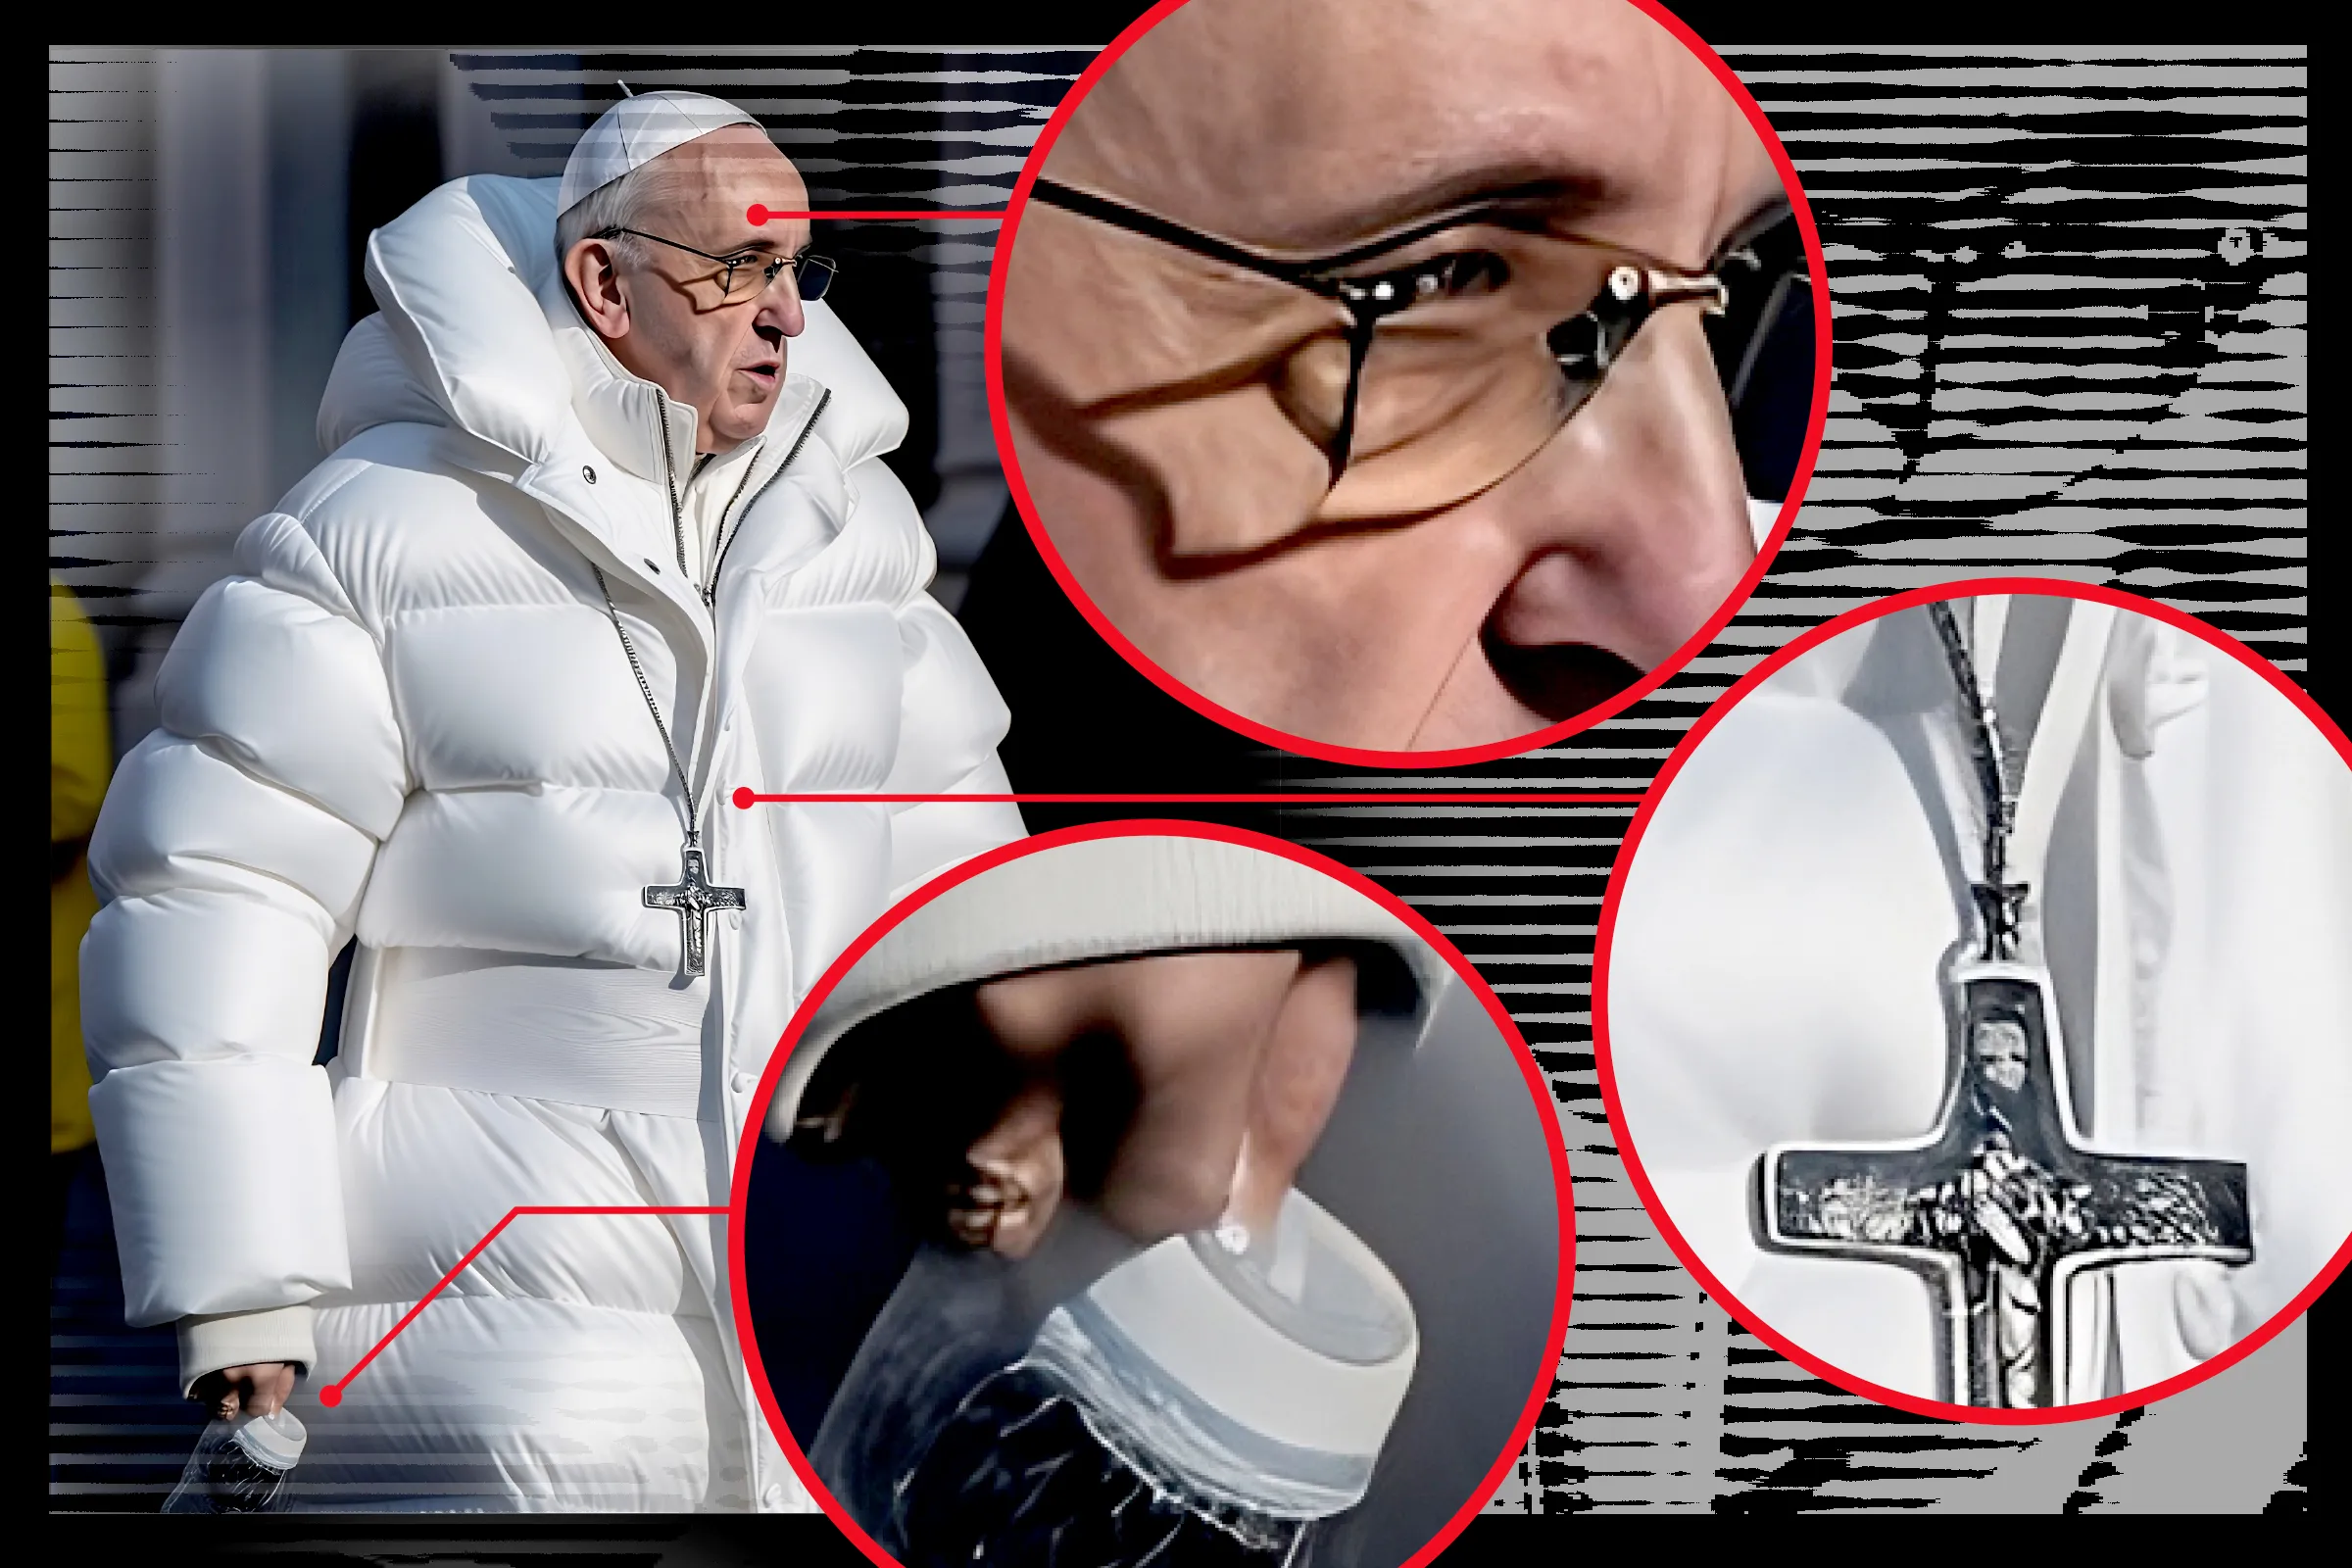
\includegraphics[width=0.7\linewidth]{slike/papa.png}
   \caption{\textit{deepfake} pape Franje s naznačenim artefaktima}
   \label{fig:report}
\end{figure}
%https://time.com/6266606/how-to-spot-deepfake-pope/
\section{GAN-ovi}
GAN-ovi su predstavljeni 2014. godine od strane Ian Goodfellowa i njegovih kolega.
Osnovna ideja iza GAN sustava jest postojanje dva glavna dijela mreže: generator i diskriminator.
Tijekom treninga, generator i diskriminator se natječu jedan protiv drugoga. Generator pokušava poboljšati svoje sposobnosti generiranja tako da vara diskriminator, dok diskriminator nastoji postati sve bolji u razlikovanju pravih podataka od lažnih. Ovaj suparnički proces dovodi do poboljšanja kvalitete generiranih podataka tijekom vremena.
\begin{figure}[H]
   \centering
   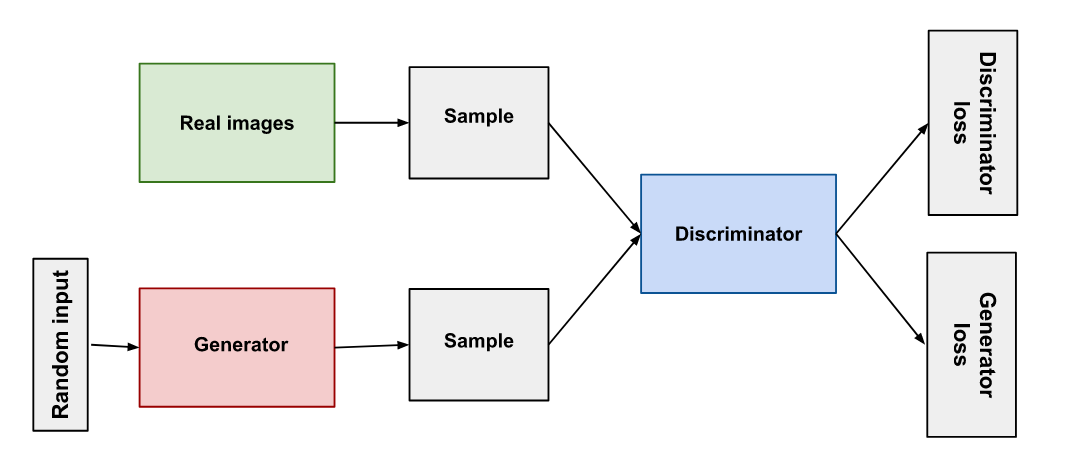
\includegraphics[width=0.7\linewidth]{slike/gan.png}
   \caption{Prikaz arhitekture GAN sustava}
   \label{fig:report}
\end{figure}
%https://developers.google.com/machine-learning/gan/gan_structure
\subsection{Generator}
Generator GAN-a je ključni dio sustava čija je zadaća stvaranje novih uzoraka ili podataka koji bi trebali biti što je moguće sličniji stvarnim primjerima iz skupa podataka na kojem je mreža trenirana. 
Na ulaz generatora dovodi se nasumični šum, a zatim se on izmjenjuje u izlaz koji nalikuje podatcima iz skupa za treniranje. Uvođenjem nasumičnog šuma te uzorkovanjem iz različitih točaka ciljne distribucije postižemo raznolikost generiranih podataka.
\begin{figure}[H]
   \centering
   \subfigure[\textit{Početak treniranja, generator jako loš}]{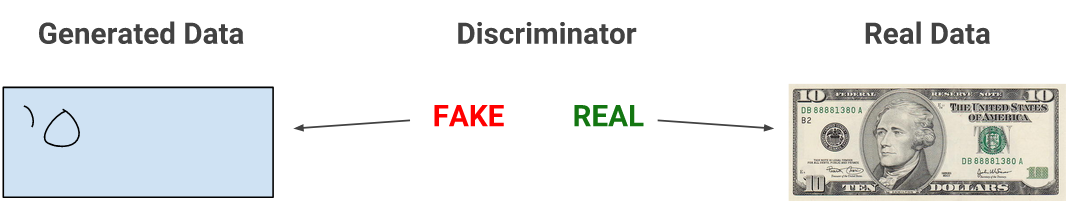
\includegraphics[width=0.75\linewidth]{slike/gan_stage1.png}}
   \subfigure[\textit{Generator iz nasumičnog ulaza počinje stvarati uvjerljiviji izlaz}]{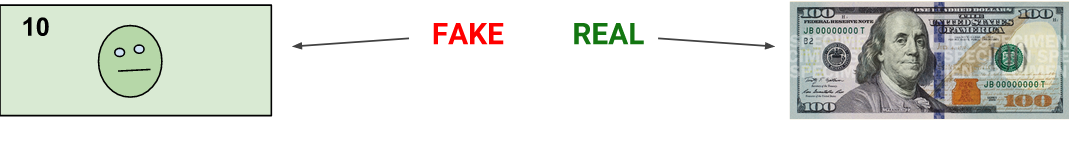
\includegraphics[width=0.75\linewidth]{slike/gan_stage2.png}}
   \subfigure[\textit{Generator zavarava diskriminator}]{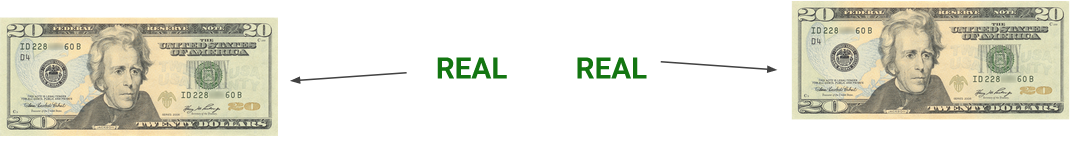
\includegraphics[width=0.75\linewidth]{slike/gan_stage3.png}}
\end{figure}
Generator dakle kreira sadržaj suparničkim pristupom, pokušavajući prevariti diskriminator, poboljšava svoj izlaz iz iteracije u iteraciju.

\subsection{Diskriminator}
Diskriminator u okviru GAN-a se jednostavno može opisati kao klasifikator, čija je osnovna zadaća razlikovanje stvarnih podataka od onih koje generira sam generator. Proces treniranja diskriminatora uključuje podatke iz dva izvora, čime se postiže njegova sposobnost prepoznavanja stvarnih i generiranih podataka. Stvarni podaci, poput autentičnih slika ljudi, služe kao pozitivni primjeri tijekom učenja. Ovi primjeri omogućuju diskriminatoru da nauči karakteristike stvarnih podataka i stvori referentnu točku za usporedbu tijekom identifikacije lažnih podataka. S druge strane, negativni primjeri dolaze iz lažnih instanci podataka koje proizvodi generator. Diskriminator tijekom treniranja razvija sposobnost razlikovanja autentičnih, stvarnih i generiranih, lažnih podataka. Ovaj proces suparništva potiče dinamički odnos između generatora i diskriminatora, čime se postiže postupna konvergencija prema visokokvalitetnim generiranim podacima.
\setcounter{subfigure}{0}

\subsection {Primjena GAN-ova za detekciju deepfake-ova}
Ideja za primjenu dolazi iz činjenice da se upravo GAN-ovi često koriste kako bi se kreirali deepfakeovi i oni sami interno pokušavaju detektirati deepfakeove pomoću svog diskiminatora. 
U nastavku ovog rada ekstraktirati ćemo diskriminator već istreniranog GAN modela, te pomoću njega pokušati označiti uvjerljive lažne sadržaje. 

%-------------------------------------------------------------------------------
\chapter{Rezultati i rasprava}
\label{pog:rezultati_i_rasprava}
Koristili smo i rekreirali arhitekturu mreže iz rada "\textit{MesoNet: a Compact Facial Video Forgery Detection Network}\cite{mesonet}". Rad predstavlja učinkovitu metodu za automatsko detektiranje uvjerljivog krivotvorenog sadržaja lica na fotografijama i videozapisima. Posebno se fokusira na dvije moguće tehnike korištene za generiranje hiperrealističkog krivotvorenog sadržaja: \textit{Deepfake} i \textit{Face2Face}. Autori rada ističu da tradicionalne tehnike forenzike slika nisu prikladne za videozapise zbog kompresije koja snažno degradira podatke. Stoga su se odlučili za slijediti pristup dubokog učenja te su predstavili dvije mreže (\textit{Meso-4} i \textit{MesoInception-4}), obje s malim brojem slojeva kako bi se bolje usredotočile na mezoskopska svojstva slika. Eksperimenti su pokazali iznimno visoku stopu uspješnosti detekcije, s više od 98\% za \textit{Deepfake} i 95\% za \textit{Face2Face}.

\begin{figure}[H]
   \centering

   \begin{minipage}[b]{0.45\linewidth}
      \subfigure[Arhitektura \textit{Meso-4} mreže \cite{mesonet}\label{fig:arhitektura}]
         {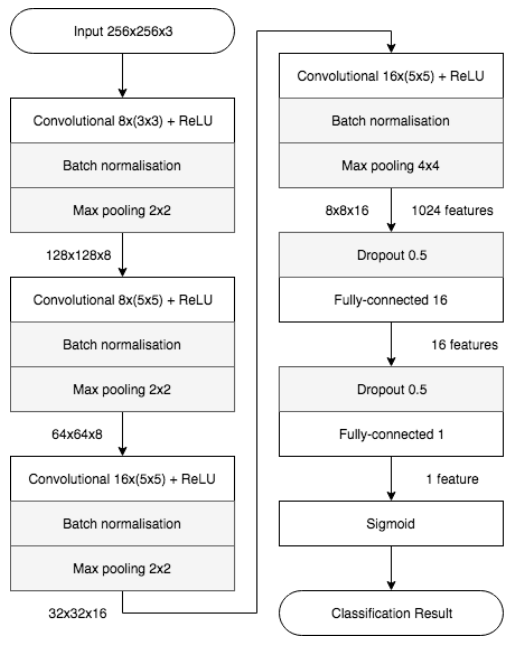
\includegraphics[width=\linewidth]{slike/arh.png}}
   \end{minipage}
   \hfill
   \begin{minipage}[b]{0.45\linewidth}
      \subfigure[Rekreiranje arhitekture \textit{Meso-4} mreže u kodu\label{fig:kod}]
         {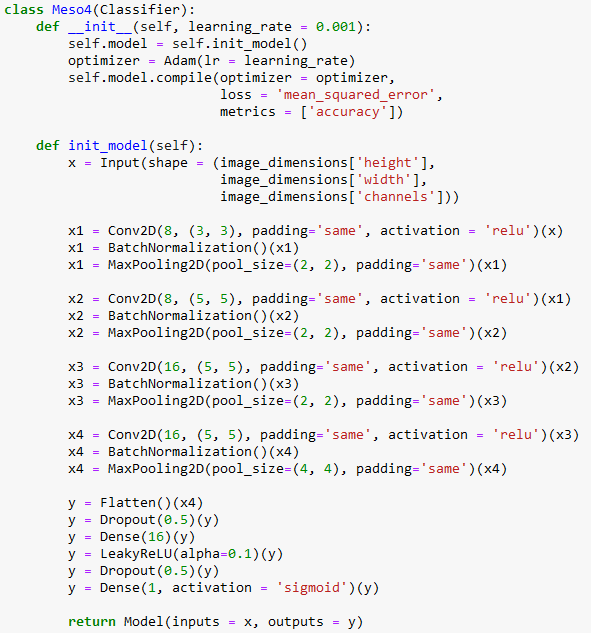
\includegraphics[width=\linewidth]{slike/kod.png}}
   \end{minipage}
   
   \caption{Mreža Meso-4}
   \label{fig:mreza}

\end{figure}

U našem kodu na slici \ref{fig:kod} rekreirali smo \textit{Meso-4} mrežu, čija se arhitektura može vidjeti na slici \ref{fig:arhitektura}\cite{mesonet}. Arhitektura mreže započinje s četiri sloja uzastopnih konvolucija i grupiranja (engl. \textit{pooling}). Za poboljšanje generalizacije, konvolucijski slojevi koriste \textit{ReLU} aktivacijske funkcije i postupak normalizacije po grupi (engl.\textit{batch normalization}), dok potpuno povezani slojevi koriste \textit{dropout} tehniku za reguliranje i poboljšanje robusnosti. Nakon što smo rekreirali arhitekturu mreže, preuzeli smo težine njihovog istreniranog modela i testirali ga na različitim fotografijama. 

Rezultati evaluacije modela pružaju uvid u njegovu sposobnost razlikovanja između stvarnih i krivotvorenih sadržaja. Na slici nniže prikazane su sljedeće vrijednosti: točni pozitivi (engl. \textit{true positives}), lažni pozitivi (engl. \textit{false positives}), točni negativi (engl. \textit{true negatives}) te lažni negativi (engl. \textit{false negatives}).

\setcounter{subfigure}{0}
\begin{figure}[H]
   \centering

   \subfigure[\textit{True positives}]{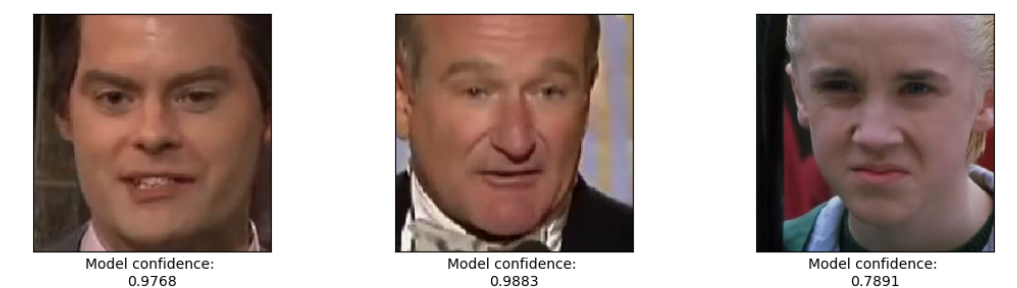
\includegraphics[width=0.75\linewidth]{slike/tp.png}}
   \subfigure[\textit{False positives}]{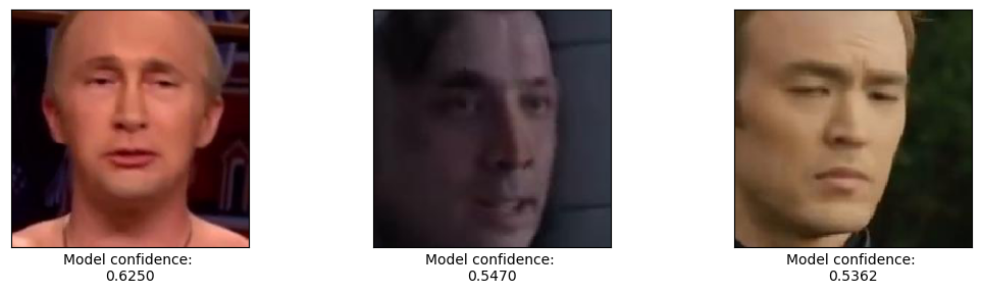
\includegraphics[width=0.75\linewidth]{slike/fp.png}}
   \subfigure[\textit{True negatives}]{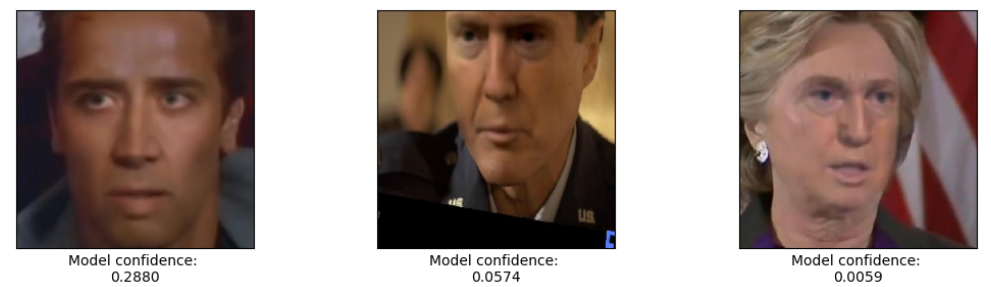
\includegraphics[width=0.75\linewidth]{slike/tn.png}}
   \subfigure[\textit{False negatives}]{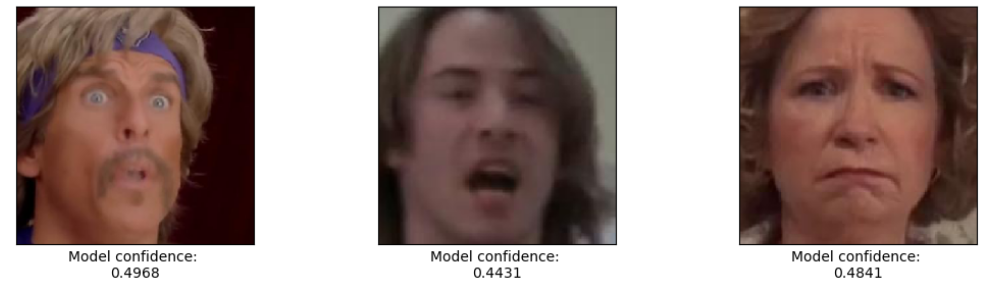
\includegraphics[width=0.75\linewidth]{slike/fn.png}}

\end{figure}

Točni pozitivi su stvarni nekrivotvoreni primjeri koje je model ispravno klasificirao, a lažni pozitivi su stvarni krivotvoreni primjera koje je model pogrešno klasificirao kao nekrivotvorene. Točni negativi su ispravno detektirani uvjerljivi krivotvoreni sadržaj, a lažni negativi su stvarni nekrivotvoreni primjeri koje je model pogrešno klasificirao kao krivotvorene. Ovi parametri pružaju cjelovitu sliku očekivane izvedbe modela u kontekstu detekcije krivotvorenog sadržaja.

Matrica zabune (engl. \textit{confusion matrix}), prikazana na slici \ref{fig:matrica}, pruža vizualnu interpretaciju prethodno objašnjenih vrijednosti. Podijeljena je na četiri kvadranta, a svaki kvadrant predstavlja različitu kombinaciju predviđenih i stvarnih klasifikacija. Gornji lijevi kvadrant sadrži točne negative (2564), a gornji desni kvadrant lažne pozitive (281). Donji lijevi kvadrant predstavlja lažne negative (513), dok donji desni kvadrant prikazuje točne pozitive (3746).

\begin{figure}[H]
   \centering
   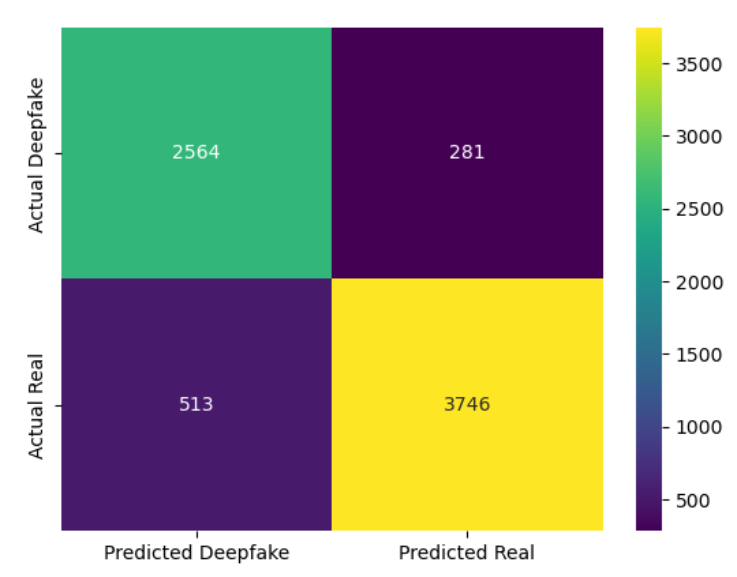
\includegraphics[width=0.7\linewidth]{slike/matrica.png}
   \caption{Matrica zabune (engl. \textit{confusion matrix})}
   \label{fig:matrica}
\end{figure}

Slika \ref{fig:report} pruža detaljan izvještaj klasifikacije, uključujući preciznost, odziv, F1-score i podršku za svaku klasu. 
Preciznost (engl. \textit{precision} mjeri točnost klasifikacije primjera, odnosno stavlja u omjer broj ispravno klasificiranih primjera određene klase s ukupnim brojem primjera predviđenih kao ta klasa. Prema klasifikacijskom izvještaju, klasifikator ima visoku razinu točnosti i preciznosti u razlikovanju između \textit{deepfake} i stvarnih fotografija, s preciznošću od 0,83 za \textit{deepfake} razred i 0,93 za \textit{real} razred.
Odziv (engl. \textit{recall}) mjeri broj pravilno identificiranih primjera određene klase u odnosu na ukupan broj primjera te klase. Mjera \textit{F1-score} harmonična je sredina preciznosti i odziva, te pruža balansiranu mjeru performansi. Iz priložene slike, primjećujemo vrlo visoke razine odziva i \textit{F1-score}a za obje klase.

\begin{figure}[H]
   \centering
   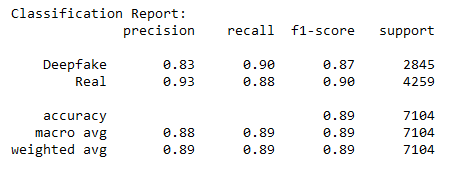
\includegraphics[width=0.7\linewidth]{slike/report.png}
   \caption{Klasifikacijski izvještaj}
   \label{fig:report}
\end{figure}

AUC-ROC krivulja na slici \ref{fig:auc} pruža grafički prikaz performansi klasifikatora u razlikovanju između dvije klase. Površina ispod krivulje (AUC) mjeri koliko dobro klasifikator razlikuje dvije klase. Što je AUC veći, to je klasifikator bolji u razlikovanju između klasa. Rezultati pokazuju značajnu površinu ispod krivulje, što ukazuje na izvrsne performanse klasifikatora u razlikovanju razreda \textit{deepfake} i \textit{real}. AUC-ROC krivulja je korisna jer omogućuje usporedbu performansi klasifikatora na različitim pragovima odlučivanja.

\begin{figure}[H]
   \centering
   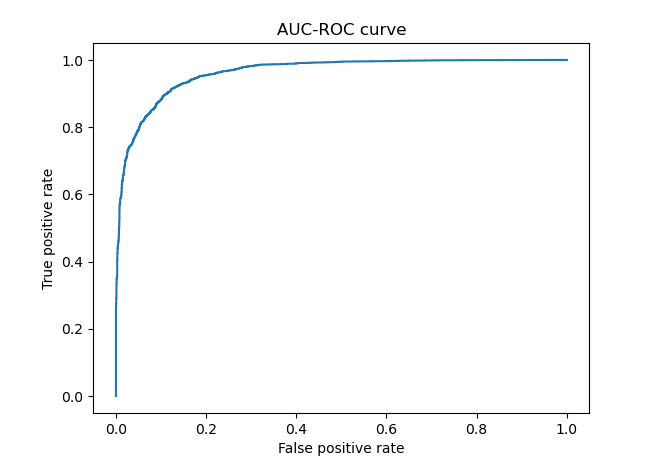
\includegraphics[width=0.7\linewidth]{slike/auc.png}
   \caption{AUC-ROC krivulja}
   \label{fig:auc}
\end{figure}

Sveobuhvatna evaluacija klasifikatora \textit{Meso-4}, temeljenog na \textit{MesoNet} arhitekturi, potvrđuje izuzetnu učinkovitost u detekciji uvjerljivog krivotvorenog sadržaja, pružajući obećavajuće perspektive za suzbijanje manipulacije sadržajem na društvenim mrežama.


%--- ZAKLJUČAK / CONCLUSION ----------------------------------------------------
\chapter{Zaključak}
Budući rad na ovom projektu uključuje izgradnju te treniranje vlastitog GAN modela, treniranje istog te ekstrakciju tako istreniranog diskriminatora. Ovako dobiveni diskriminator može biti iskorišten u raznim programskim rješenjima koja bi u stvarnom vremenu pregledavale sadržaje na društvenim mrežama, 
detektirale krivotvoreni sadržaj i upozoravale korisnike na pojavu deepfakeova. Smatramo da bi navedena primjena učinila društvene mreže sigurnijima, reducirala širenje dezinformacija i smanjila potencijal za malicioznu uporabu uvjerljivo krivotvorenih sadržaja bez ograničavanja te tehnologije koja ima izrazito širok spektar primjena. 
\label{pog:zakljucak}



%--- LITERATURA / REFERENCES ---------------------------------------------------

% Literatura se automatski generira / References are automatically generated
% Upiši ime BibTeX datoteke bez .bib nastavka / Enter the name of the BibTeX file without .bib extension
\bibliography{literatura}


%--- PRIVITCI / APPENDIX -------------------------------------------------------
\chapter{Privitci}


\end{document}
